\section{Radiation pattern}

\subsection{Gain and Directivity}
The gain of the dipole is represented in dB as the polar plot of the $\vec{E}$
Field in Figure~\ref{fig:pgain} generated by FEKO.

\begin{figure}[h!]
  \centering
  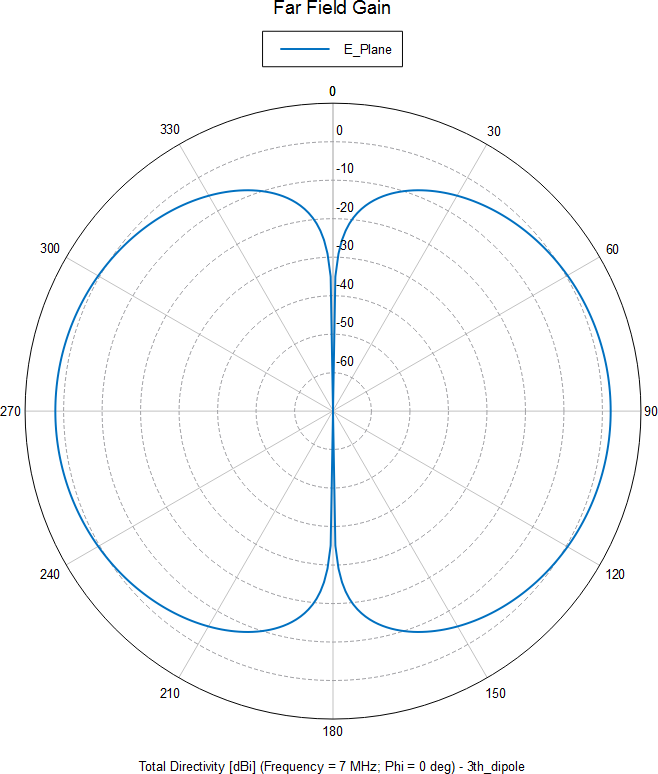
\includegraphics[width=0.40\textwidth]{./img/polgain.png}
  \caption{Dipole Gain}
  \label{fig:pgain}
\end{figure}
The directivity of a dipole radiation pattern is omnidirectional, with a null
at the point where $\theta=0^\circ$. This is more readily seen in the full 3D
far field plot in Figure~\ref{fig:3D}. When $\theta=90^\circ$, the gain is at
its peak value. The $\vec{H}$ field is normal to the dipole and is perfectly
circular. This simplifies analysis, as any slice of the $\vec{E}$ field is
equivalent to any other slice.

\begin{figure}[h!]
  \centering
  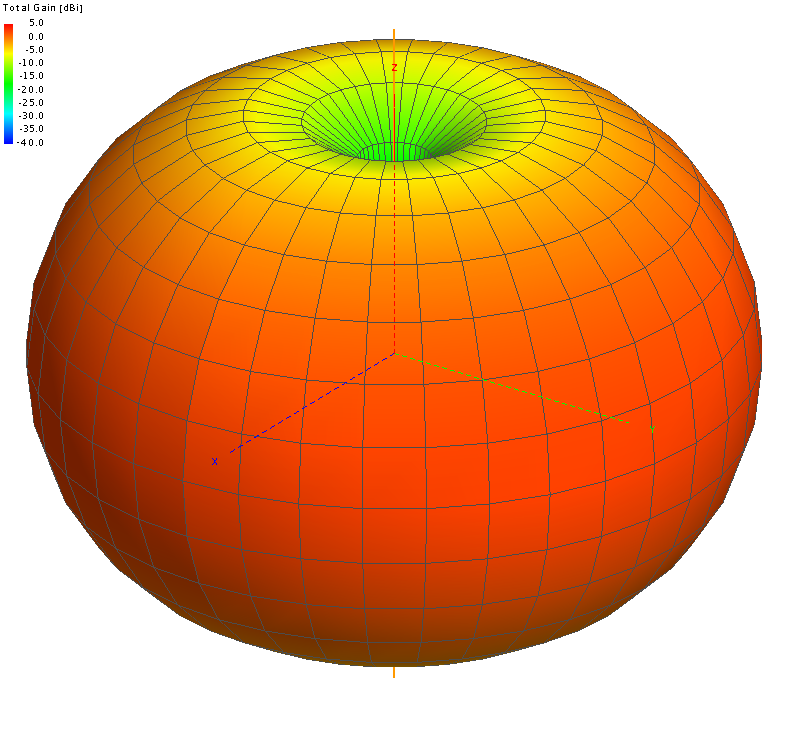
\includegraphics[width=0.38\textwidth]{./img/Gain.png}
  \caption{Dipole Radiation Pattern in 3D}
  \label{fig:3D}
\end{figure}

\subsection{3dB beamwidth}

The 3dB beamwidth, or, the angle where most of the power is transmitted was
found using FEKO, and the plot is in Figure~\ref{fig:3dbbeamw}.


\begin{figure}[h!]
  \centering
  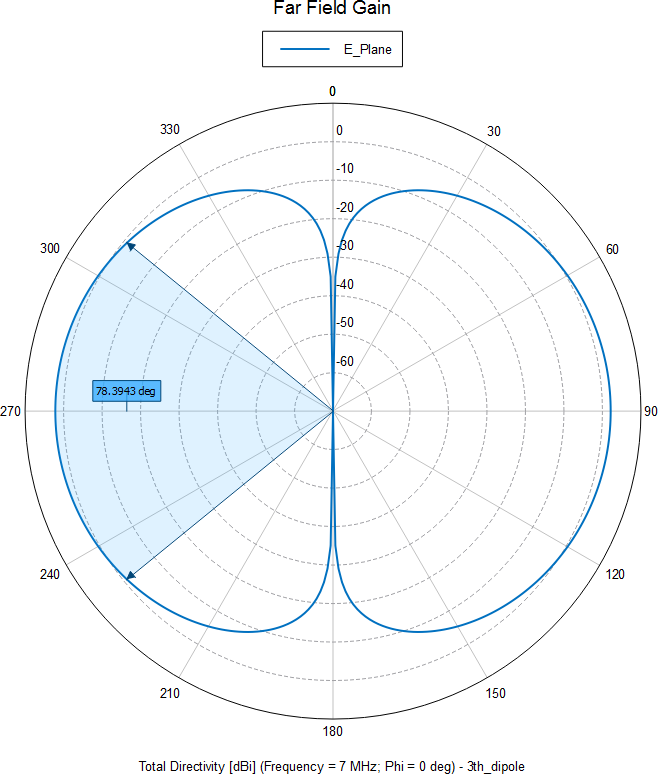
\includegraphics[width=0.40\textwidth]{./img/3dbeamw.png}
  \caption{Dipole 3dB Beamwidth}
  \label{fig:3dbbeamw}
\end{figure}
